
%% bare_conf.tex
%% V1.4b
%% 2015/08/26
%% by Michael Shell
%% See:
%% http://www.michaelshell.org/
%% for current contact information.
%%
%% This is a skeleton file demonstrating the use of IEEEtran.cls
%% (requires IEEEtran.cls version 1.8b or later) with an IEEE
%% conference paper.
%%
%% Support sites:
%% http://www.michaelshell.org/tex/ieeetran/
%% http://www.ctan.org/pkg/ieeetran
%% and
%% http://www.ieee.org/

%%*************************************************************************
%% Legal Notice:
%% This code is offered as-is without any warranty either expressed or
%% implied; without even the implied warranty of MERCHANTABILITY or
%% FITNESS FOR A PARTICULAR PURPOSE!
%% User assumes all risk.
%% In no event shall the IEEE or any contributor to this code be liable for
%% any damages or losses, including, but not limited to, incidental,
%% consequential, or any other damages, resulting from the use or misuse
%% of any information contained here.
%%
%% All comments are the opinions of their respective authors and are not
%% necessarily endorsed by the IEEE.
%%
%% This work is distributed under the LaTeX Project Public License (LPPL)
%% ( http://www.latex-project.org/ ) version 1.3, and may be freely used,
%% distributed and modified. A copy of the LPPL, version 1.3, is included
%% in the base LaTeX documentation of all distributions of LaTeX released
%% 2003/12/01 or later.
%% Retain all contribution notices and credits.
%% ** Modified files should be clearly indicated as such, including  **
%% ** renaming them and changing author support contact information. **
%%*************************************************************************


% *** Authors should verify (and, if needed, correct) their LaTeX system  ***
% *** with the testflow diagnostic prior to trusting their LaTeX platform ***
% *** with production work. The IEEE's font choices and paper sizes can   ***
% *** trigger bugs that do not appear when using other class files.       ***                          ***
% The testflow support page is at:
% http://www.michaelshell.org/tex/testflow/



\documentclass[conference]{IEEEtran}
% Some Computer Society conferences also require the compsoc mode option,
% but others use the standard conference format.
%
% If IEEEtran.cls has not been installed into the LaTeX system files,
% manually specify the path to it like:
% \documentclass[conference]{../sty/IEEEtran}





% Some very useful LaTeX packages include:
% (uncomment the ones you want to load)


% *** MISC UTILITY PACKAGES ***
%
%\usepackage{ifpdf}
% Heiko Oberdiek's ifpdf.sty is very useful if you need conditional
% compilation based on whether the output is pdf or dvi.
% usage:
% \ifpdf
%   % pdf code
% \else
%   % dvi code
% \fi
% The latest version of ifpdf.sty can be obtained from:
% http://www.ctan.org/pkg/ifpdf
% Also, note that IEEEtran.cls V1.7 and later provides a builtin
% \ifCLASSINFOpdf conditional that works the same way.
% When switching from latex to pdflatex and vice-versa, the compiler may
% have to be run twice to clear warning/error messages.






% *** CITATION PACKAGES ***
%
%\usepackage{cite}
% cite.sty was written by Donald Arseneau
% V1.6 and later of IEEEtran pre-defines the format of the cite.sty package
% \cite{} output to follow that of the IEEE. Loading the cite package will
% result in citation numbers being automatically sorted and properly
% "compressed/ranged". e.g., [1], \cite{seznec2007tage}, \cite{calder1997evidence}, \cite{lee1995branch}, \cite{jimenez2001dynamic}, \cite{jimenez2003fast} without using
% cite.sty will become [1], \cite{calder1997evidence}, \cite{jimenez2001dynamic}--\cite{lee1995branch}, \cite{seznec2007tage} using cite.sty. cite.sty's
% \cite will automatically add leading space, if needed. Use cite.sty's
% noadjust option (cite.sty V3.8 and later) if you want to turn this off
% such as if a citation ever needs to be enclosed in parenthesis.
% cite.sty is already installed on most LaTeX systems. Be sure and use
% version 5.0 (2009-03-20) and later if using hyperref.sty.
% The latest version can be obtained at:
% http://www.ctan.org/pkg/cite
% The documentation is contained in the cite.sty file itself.






% *** GRAPHICS RELATED PACKAGES ***
%
\ifCLASSINFOpdf
  % \usepackage[pdftex]{graphicx}
  % declare the path(s) where your graphic files are
  % \graphicspath{{../pdf/}{../jpeg/}}
  % and their extensions so you won't have to specify these with
  % every instance of \includegraphics
  % \DeclareGraphicsExtensions{.pdf,.jpeg,.png}
\else
  % or other class option (dvipsone, dvipdf, if not using dvips). graphicx
  % will default to the driver specified in the system graphics.cfg if no
  % driver is specified.
  % \usepackage[dvips]{graphicx}
  % declare the path(s) where your graphic files are
  % \graphicspath{{../eps/}}
  % and their extensions so you won't have to specify these with
  % every instance of \includegraphics
  % \DeclareGraphicsExtensions{.eps}
\fi
\usepackage{algorithm}
\usepackage{algpseudocode}
\usepackage{amsmath}
\usepackage{amsmath,amssymb,amsthm,latexsym,paralist, booktabs}
\usepackage{url}
\usepackage[pdftex]{graphicx}
% default pic path
\usepackage{bm}
\usepackage{mathtools}
\let\oldvec\vec
\renewcommand{\vec}[1]{\oldvec{\mathit{#1}}}
\newcommand{\mat}[1]{\mathbf{#1}} % undergraduate algebra version
\newcommand{\parallelsum}{\mathbin{\!/\mkern-5mu/\!}}
\graphicspath{{pics/}}
\usepackage{subfigure}

\usepackage{listings}
\usepackage{color} %red, green, blue, yellow, cyan, magenta, black, white
\definecolor{mygreen}{RGB}{28,172,0} % color values Red, Green, Blue
\definecolor{mylilas}{RGB}{170,55,241}

%\newcommand{\mat}[1]{\bm{\mathit{#1}}}




% *** Do not adjust lengths that control margins, column widths, etc. ***
% *** Do not use packages that alter fonts (such as pslatex).         ***
% There should be no need to do such things with IEEEtran.cls V1.6 and later.
% (Unless specifically asked to do so by the journal or conference you plan
% to submit to, of course. )


% correct bad hyphenation here
\hyphenation{op-tical net-works semi-conduc-tor}


\begin{document}
\lstset{language=Matlab,%
    %basicstyle=\color{red},
    breaklines=true,%
    morekeywords={matlab2tikz},
    keywordstyle=\color{blue},%
    morekeywords=[2]{1}, keywordstyle=[2]{\color{black}},
    identifierstyle=\color{black},%
    stringstyle=\color{mylilas},
    commentstyle=\color{mygreen},%
    showstringspaces=false,%without this there will be a symbol in the places where there is a space
    numbers=left,%
    numberstyle={\tiny \color{black}},% size of the numbers
    numbersep=9pt, % this defines how far the numbers are from the text
    emph=[1]{for,end,break},emphstyle=[1]\color{red}, %some words to emphasise
    %emph=[2]{word1,word2}, emphstyle=[2]{style},    
}
%
% paper title
% Titles are generally capitalized except for words such as a, an, and, as,
% at, but, by, for, in, nor, of, on, or, the, to and up, which are usually
% not capitalized unless they are the first or last word of the title.
% Linebreaks \\ can be used within to get better formatting as desired.
% Do not put math or special symbols in the title.
\title{CSCE 643 Multi-View Geometry CV\\
Project II}


% author names and affiliations
% use a multiple column layout for up to three different
% affiliations

% conference papers do not typically use \thanks and this command
% is locked out in conference mode. If really needed, such as for
% the acknowledgment of grants, issue a \IEEEoverridecommandlockouts
% after \documentclass

% for over three affiliations, or if they all won't fit within the width
% of the page, use this alternative format:
%
%\author{\IEEEauthorblockN{Michael Shell\IEEEauthorrefmark{1},
%Homer Simpson\IEEEauthorrefmark{2},
%James Kirk\IEEEauthorrefmark{3},
%Montgomery Scott\IEEEauthorrefmark{3} and
%Eldon Tyrell\IEEEauthorrefmark{4}}
%\IEEEauthorblockA{\IEEEauthorrefmark{1}School of Electrical and Computer Engineering\\
%Georgia Institute of Technology,
%Atlanta, Georgia 30332--0250\\ Email: see http://www.michaelshell.org/contact.html}
%\IEEEauthorblockA{\IEEEauthorrefmark{2}Twentieth Century Fox, Springfield, USA\\
%Email: homer@thesimpsons.com}
%\IEEEauthorblockA{\IEEEauthorrefmark{3}Starfleet Academy, San Francisco, California 96678-2391\\
%Telephone: (800) 555--1212, Fax: (888) 555--1212}
%\IEEEauthorblockA{\IEEEauthorrefmark{4}Tyrell Inc., 123 Replicant Street, Los Angeles, California 90210--4321}}




% use for special paper notices
%\IEEEspecialpapernotice{(Invited Paper)}




% make the title area
\maketitle
% As a general rule, do not put math, special symbols or citations
% in the abstract

% no keywords




% For peer review papers, you can put extra information on the cover
% page as needed:
% \ifCLASSOPTIONpeerreview
% \begin{center} \bfseries EDICS Category: 3-BBND \end{center}
% \fi
%
% For peerreview papers, this IEEEtran command inserts a page break and
% creates the second title. It will be ignored for other modes.
\IEEEpeerreviewmaketitle


\section{Calibrate Lens Distortion}
A basic assumption in camera geometry study is that a linear model is an accurate model of the imaging process, i.e., world point, image point and optical center point are collinear and world lines are imaged as lines and so on. However, this might not be true for real lens in the world. Radial distortion is a typical deviation that real lens might have, we need to correct image measurements to those that should be obtained under a perfect linear camera action.

\subsection{Problem Formulation}
Suppose $(\tilde{x}, \tilde{y})$ is the ideal image position that obeys linear projection (under perfect lens settings), $(x_d, y_d)$ to be the actual image position after the effects of radial distortion, $\tilde{r} = \sqrt{\tilde{x^2} + \tilde{y^2}}$ is the radial distance from the center of radial distortion, $L(\tilde{r})$ is a function of radius $\tilde{r}$ as the distortion factor. 

For the coordinates of point under non-distorted pinhole projection $(\tilde{x}, \tilde{y})$ (in units of focal-length), we have:
\begin{equation}
	(\tilde{x}, \tilde{y}, 1)^T = [ I| \mat{0}] \mat{x}_{cam}
\end{equation}

where $\mat{x}_{cam}$ is the 3D point in camera coordinates and it is related to world coordinates as follows:
\begin{equation}
	\mat{x}_{cam} = \begin{bmatrix}
				R & -R\tilde{\mat{C}}\\
				0 & 1
			\end{bmatrix}
			\begin{pmatrix}
				X\\
				Y\\
				Z\\
				1
			\end{pmatrix}
			=\begin{bmatrix}
				R & -R\tilde{\mat{C}}\\
				0 & 1
			\end{bmatrix}\mat{x}
\end{equation}

Now we can easily model the radial distortion by introducing the function of $\tilde{r}$:
\begin{equation}
	\begin{pmatrix}
		x_d\\
		y_d
	\end{pmatrix}
	=L(\tilde{r})\begin{pmatrix}
		\tilde{x}\\
		\tilde{y}
	\end{pmatrix}
\end{equation}

If we dig into a single point coordinate $(x, y)$, we have:
\begin{equation}
\begin{split}
	\tilde{x} = x_c + L(r)(x-x_c)\\
	\tilde{y} = y_c + L(r)(y-y_c)
\end{split}
\end{equation}
where $(x_c, y_c)$ is center of the image, $(\tilde{x}, \tilde{y})$ is the coordinates after correcting radial distortion. Also be noticed that $r$ can is the radius from center of the image to the measured coordinates, which can be solved by:
\begin{equation}
	r^2 = (x-x_c)^2 + (y-y_c)^2
\end{equation}

\subsection{Distortion function and image center}
Now let's talk about the choice of function $L(r)$ and center of image $(x_c, y_c)$. According to the textbook, $L(r)$ is only defined for positive $r$ and $L(0) = 1$. We can use Taylor expansion as an approximation of the distortion function:
\begin{equation}
	L(r) = 1 + k_1r + k_2r^2 + k_3r^3 + \dots
\end{equation}

For image center $(x_c, y_c)$, we often use principal point though it might not reside in the exact same location. On choosing the distortion function for this project, we did a tradeoff consideration. Apparently if we have higher order Taylor expansion for distortion function, we can get better correcting results, however, as the camera we are actually using is really good (though it is a relatively old model, modern cameras are generally good enough and generates very little distortion), we decided to choose $L(r) = 1 + k_1r + k_2r^2$ as our distortion function.
The intuition behind this is that typically we choose higher order of distortion function as the degree of distortion increases, in our case the distortion is even ignorable thus we use a typical 2-order function to deal with our case.

\subsection{Distortion function minimization}
Similar as the minimization process we have done in the previous projects, here we need to minimize the geometric distance between predicted coordinates (by using $L(r)$) and measured coordinates. This can be done by exploiting the colinearity of points on the same line. In our project, we use the checker board image captured by our camera for lens distortion correction. The basic idea is that we can easily identify corner points on checker board and they naturally form parallel and perpendicular lines. If we determine a straight line using two corner points on the line, then all the other corner points along the line should be on the line if without radial distortion. Let's consider a simple scenario, suppose we have $\mat{A}, \mat{B}, \mat{D}$ on same line of a checker board, and the image center is $\mat{C}$, then we can do cross product to solve the crossing product of $\vec{AB}$ and $\vec{CD}$ to get $\mat{D}^{\prime} = \vec{AB}\times \vec{CD}$, due to the radial distortion we have $\mat{D} \neq \mat{D}^\prime$. If we apply $L(r)$ for the measured $D$ to get corrected coordinates $\hat{\mat{D}}$, we want to find a function that minimizes $d(\hat{\mat{D}}, \mat{D}^\prime)$. This is now reduced to a simple minimization problem of geometric distance like we did before, we can construct the corresponding error function based on discussions above and use non linear solver in MATLAB to get function $L(r)$ that does the required minimization.

\subsection{Experiment Results}
To evaluate the performance of our approach, we started an experiment. We fixed the focal length of our camera by turning off the auto focus function and stick a checker board on the wall as the object we use for calibration, the original colored photo we get from the camera is shown in Figure \ref{single}.

\begin{figure}[htbp]
\begin{center}
\includegraphics[width=\linewidth]{single.jpg} 
\end{center}	   
\caption{The original colored picture we used for lens undistortion}\label{single}
\end{figure}

Then we grayize the photo and then use corner function provided by MATLAB to find out the corner points, the result we got from here is shown in Figure \ref{p_choice}. We then do the following steps:
\begin{itemize}
	\item Specify two perpendicular lines we want to use for this calibration.
	\item Identify all the corner points from the image.
	\item Compute the line through cross product of two end points.
	\item Compute the lines from image center to each point on those perpendicular lines, we call them lines to center.
	\item Use cross product to calculate the interceptions between two perpendicular lines and lines to center.
	\item Now we can calculate geometric distance between interceptions and measured points, we further assume $L(r) = 1 + k_1r + k_2r^2$ and use \emph{lsqnonlin} with LM option to get the $k$ that minimizes the geometric distance.
	\item After solving $L(r)$ function, we use a function for undistorting image which leverages the $L(r)$ function to remove the distortion of image.
\end{itemize}
The result after removing the distortion is also provided in Figure \ref{undistorted}. Notice that though there is no significant different between two images due to the fact that there are few radial distortion in our camera lens, we refer readers to display the original undistorted image and compare it to the original one, we can still notice changes this way.
\begin{figure*}[!hbpt]
  \subfigure[Grayized image with corner markers]{
\label{p_choice} %% label for second subfigure
\includegraphics[width=0.49\linewidth]{marked_orig.png}}
 \subfigure[The image after removing lens distortion]{
    \label{undistorted} %% label for first subfigure
    \includegraphics[width=0.49\linewidth]{undistorted.jpg}}
  \caption{Remove lens distortion}
  \label{remove_distort} %% label for entire figure
\end{figure*}


%\begin{figure*}[!hbpt]
%  \subfigure[Original source image(the image we wanna transform)]{
%\label{fig1} %% label for second subfigure
%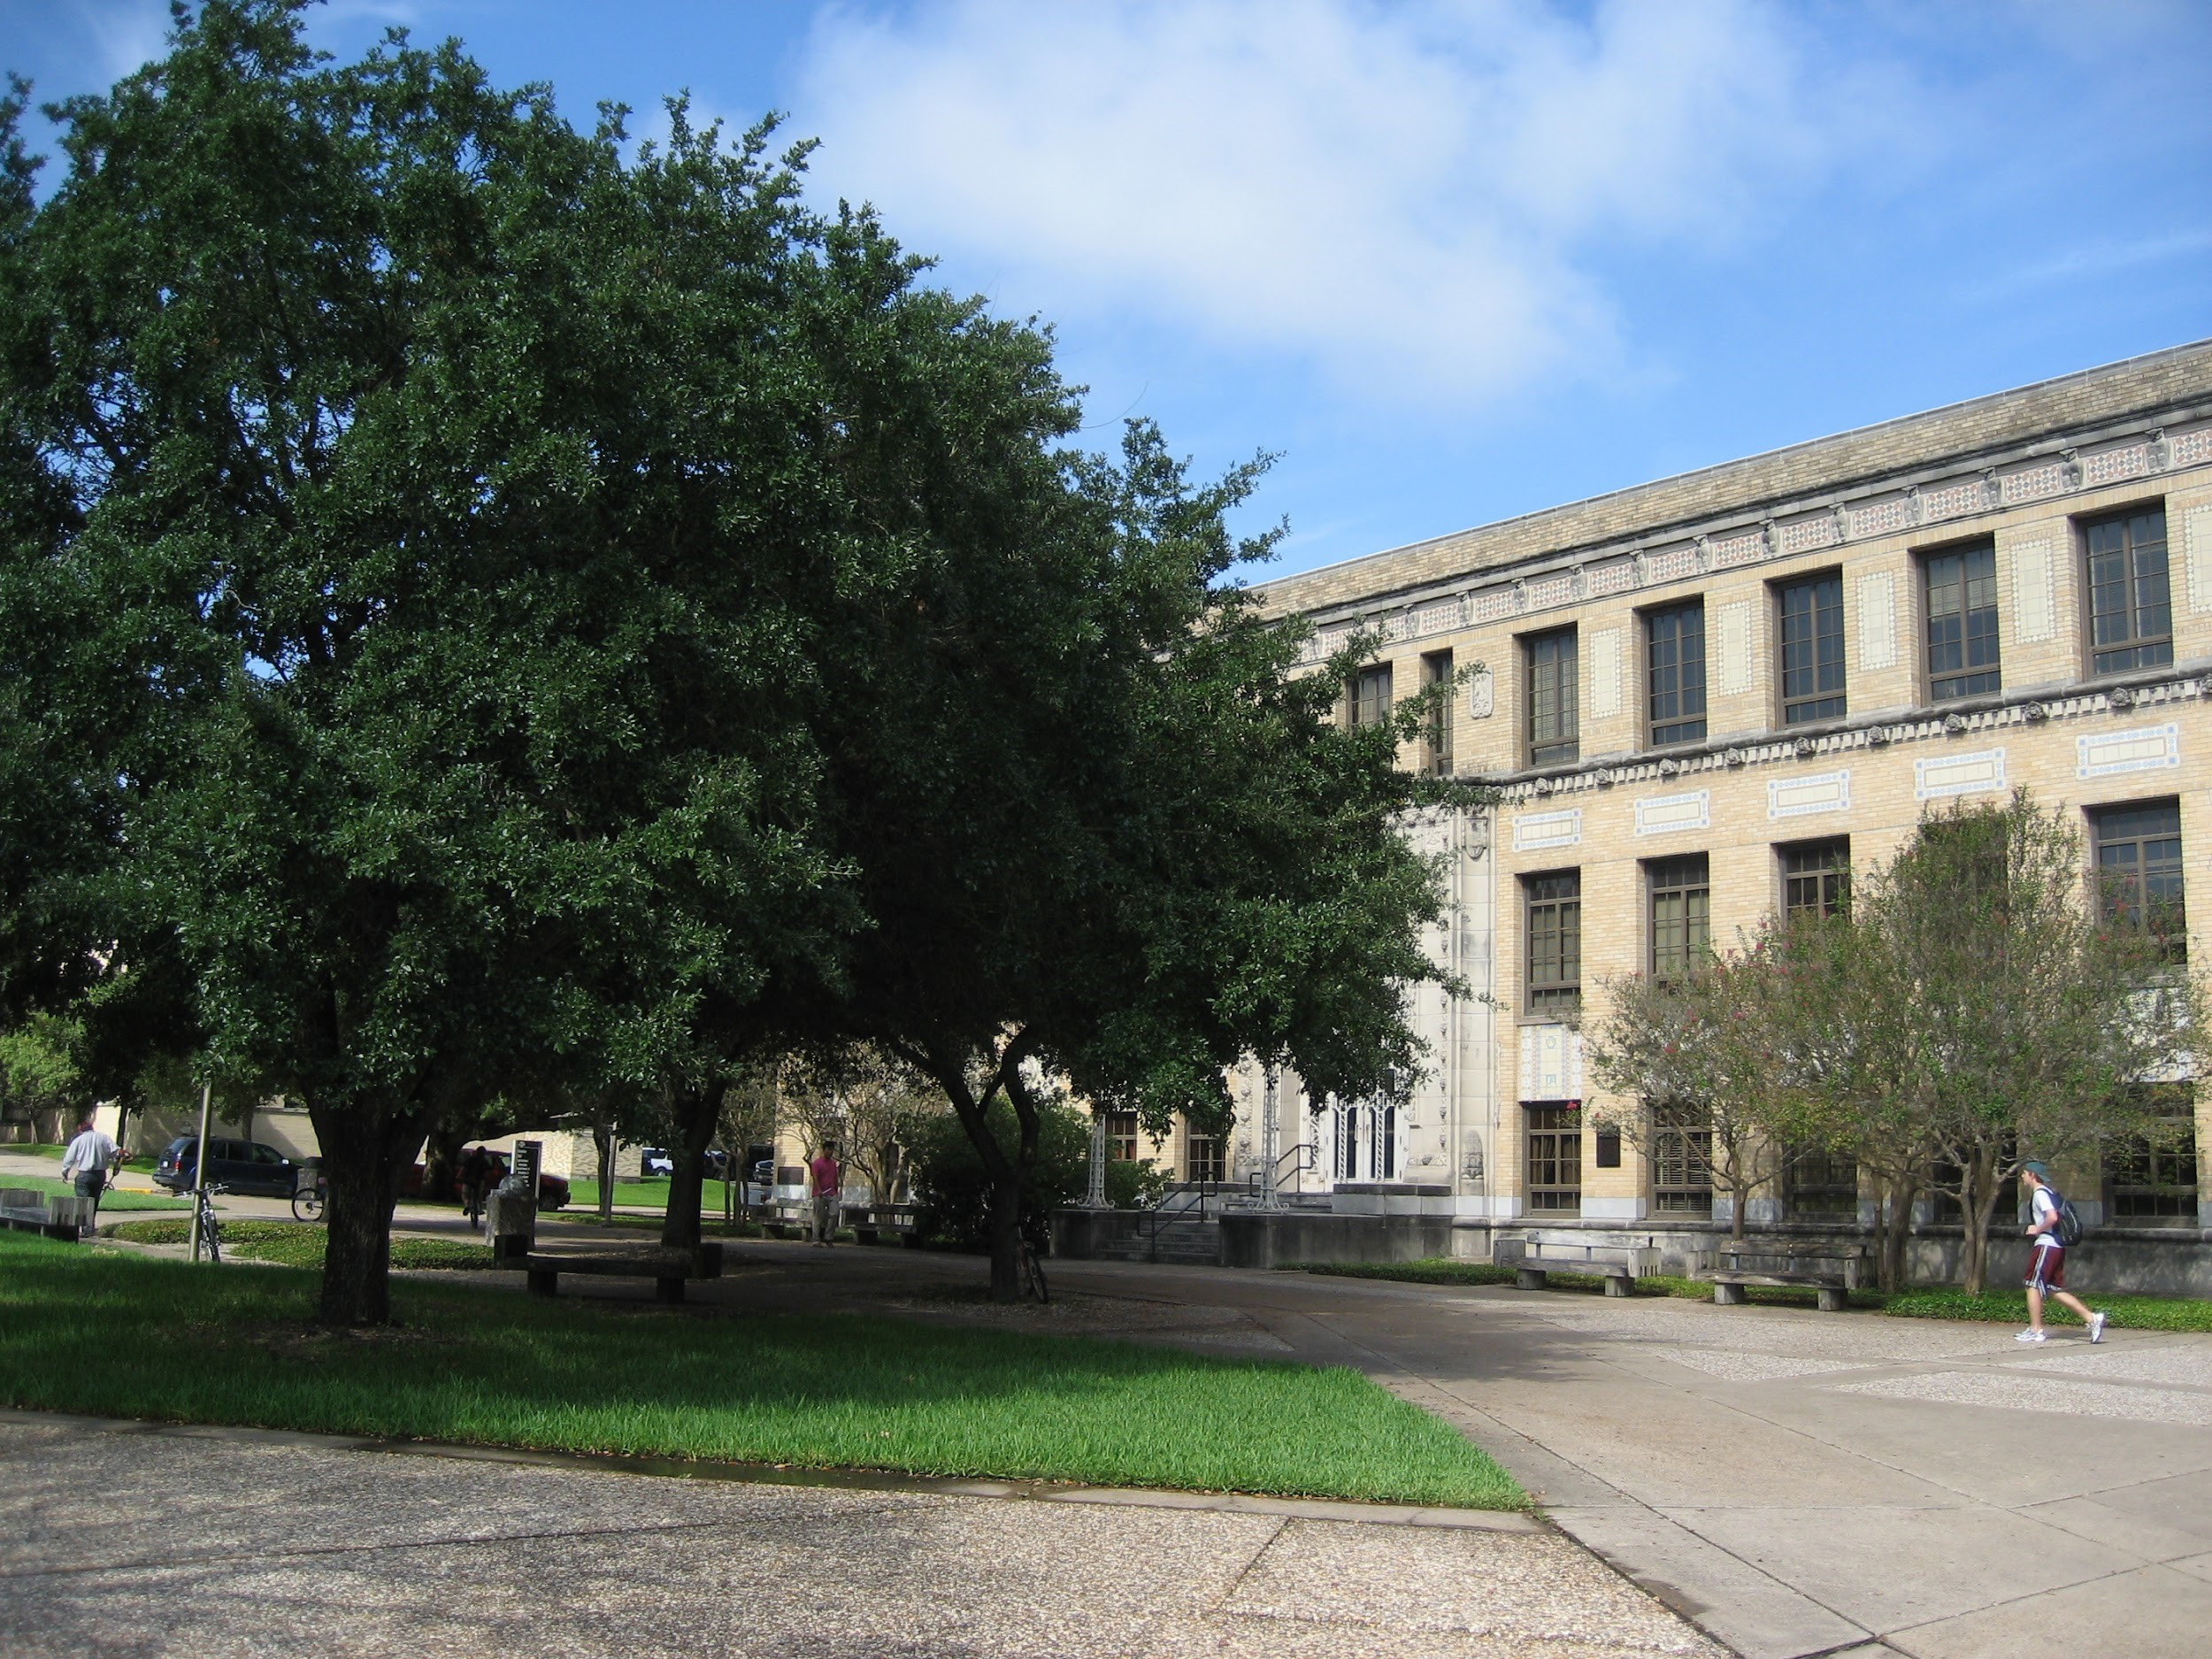
\includegraphics[width=0.49\linewidth]{fig_1.jpg}}
% \subfigure[The original target image(target image space we use for panorama)]{
%    \label{fig2} %% label for first subfigure
%    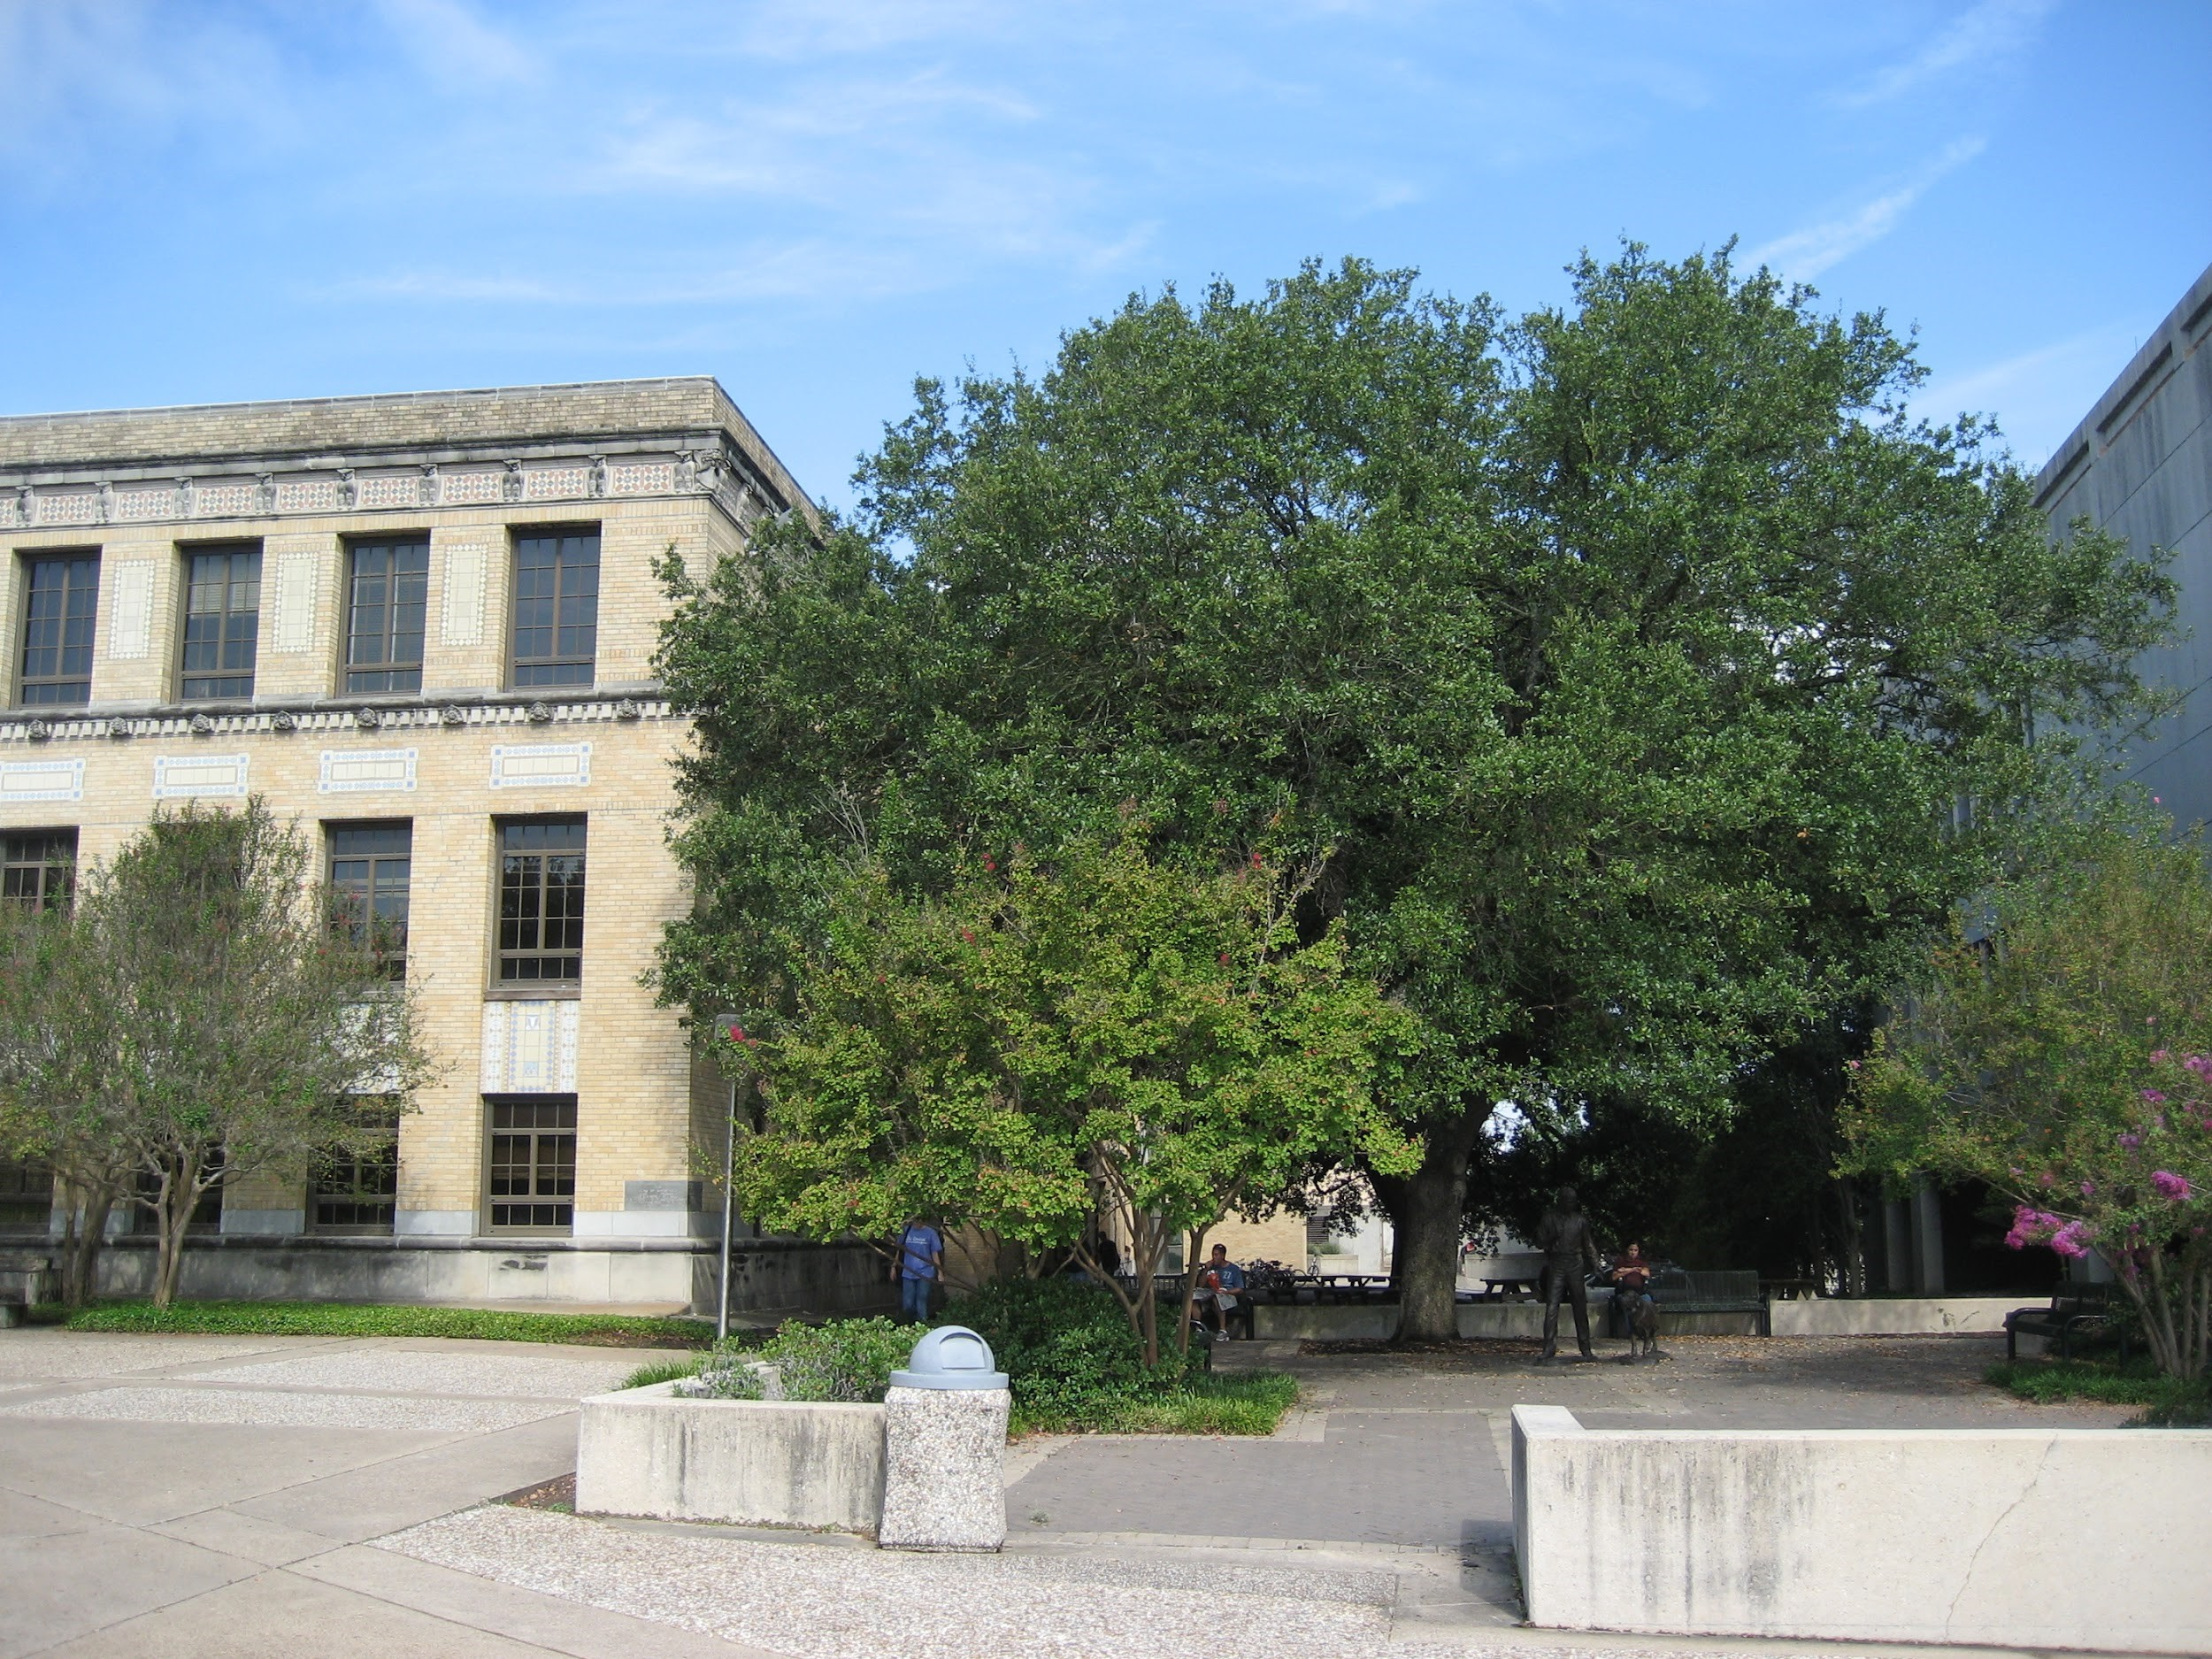
\includegraphics[width=0.49\linewidth]{fig_2.jpg}}
%  \caption{Original images}
%  \label{org_img} %% label for entire figure
%\end{figure*}

%\begin{figure}[htbp]
%\begin{center}
%\includegraphics[width=\linewidth]{pure_dlt.jpg} 
%\end{center}	   
%\caption{Panorama formed by result of pure DLT}\label{pure_dlt}
%\end{figure}

\section{Camera Calibration}
Recall from projects before, we have implemented DLT approach for finding the transformation homography from one image to another. Now in the camera calibration process, we can use similar methods, let's first adapt the original DLT approach and normalization process to camera calibration. 
\subsection{DLT Foundation}
In the simplest DLT approach, we first transform the homogeneous equation given in equation 7 as follows:
\begin{equation}
	\mat{x}_i \times \mat{P}\mat{X}_i = \mat{0}
\end{equation}
Where $\mat{P}$ is the camera matrix and can be decomposed into combination of vectors like:
\begin{equation}
	\mat{P} = \begin{pmatrix}
				\mat{p_1}\\
				\mat{p_2}\\
				\mat{p_3}
		       \end{pmatrix}
\end{equation}
Then we can rewrite equation 7 into the following form:
\begin{equation}
	\mat{P}\mat{X}_i =
	\begin{pmatrix}
		\mat{p}_1\mat{X}_i\\
		\mat{p}_2\mat{X}_i\\
		\mat{p}_3\mat{X}_i
	\end{pmatrix}
\end{equation}
Suppose the coordinates of the set of points we have are:
\begin{equation}
	\begin{split}
		\mat{x}_i = (x_i, y_i, z_i)
	\end{split}
\end{equation}
As we have $\mat{p}_i\mat{X}_i = \mat{X}_i^T \mat{p}_j^T$, we can further get the following simultaneous linear equations set:
\begin{equation}
	\begin{bmatrix}
		\mat{0}^T & -z_i\mat{X}_i^T & y_i\mat{X}_i^T\\
		z_i\mat{X}_i^T & \mat{0}^T & -x_i\mat{X}_i^T\\
		-y_i\mat{X}_i^T & x_i\mat{X}_i^T & \mat{0}^T
	\end{bmatrix}
	\begin{pmatrix}
		\mat{p}_1^T\\
		\mat{p}_2^T\\
		\mat{p}_3^T
	\end{pmatrix} = \mat{0}
\end{equation}

Be noticed that different from the math we did before in last project, here $\mat{X}_i$ is a 4D coordinates and $p_i$ also contains 4 entries. 
Since we can obtain the 3rd row of the left matrix above using by combining first two rows up to scale, we can safely prune equation 7 to only preserve the linearly independent first two rows in that matrix and obtain:
\begin{equation}
	\mat{A}
	\mat{p} = \mat{0}
\end{equation}
where
\begin{equation}
	\mat{A} = 
	\begin{bmatrix}
		\mat{0}^T & -z_i\mat{X}_i^T & y_i\mat{X}_i^T\\
		z_i\mat{X}_i^T & \mat{0}^T & -x_i\mat{X}_i^T\\
		-y_i\mat{X}_i^T & x_i\mat{X}_i^T & \mat{0}^T
	\end{bmatrix},
	\mat{p} = 
	\begin{pmatrix}
		\mat{p}_1^T\\
		\mat{p}_2^T\\
		\mat{p}_3^T
	\end{pmatrix}
\end{equation}
As we know:
\begin{equation}
	\mat{P} = 
	\begin{pmatrix}
		\mat{p}_1\\
		\mat{p}_2\\
		\mat{p}_3
	\end{pmatrix}
	=
	\begin{bmatrix}
		p_1 & p_2 & p_3 & p_4\\
		p_5 & p_6 & p_7 & p_8\\
		p_9 & p_{10} & p_{11} & p_{12}
	\end{bmatrix}
\end{equation}

Now we have come to the point that is very similar to what we have done before in Project 1. After dehomogenization, the equation 12 we get is actually a equation with 11 unknowns in $\mat{p}$ (11 DoFs) which we can solve exactly if we have $5\frac{1}{2}$ point pairs (every point pair provide 2 equations), to get the homography we can do as the followings:
\begin{itemize}
	\item If we have exact $5\frac{1}{2}$ point correspondences (which means the we can only know one of the coordinate for sixth points) in both images, we can solve equation 12 to get an exact solution, but as there might be some noises in both images, it could lead to very bad results.
	\item We can also solve this equation is we can find more point correspondence to get so-called overdetermined solution through singular value decomposition (SVD), that way we should get more accurate results since we are provided with more information in the image.
\end{itemize}

\subsection{Normalized DLT}
\subsubsection{2D Image Frame Normalization}
Similar to the DLT part we did in finding transformation homography between two images, it's sometimes very important to carry out coordinates normalization to provide better homography (camera matrix in current case). $\mat{x}_i$ is in the same dimension as before, thus we can normalize it using previous method, i.e., the points should be translated so that centroid of all points is at the origin and we also need to scale them so that their RMS (root-mean-squared) distance from origin is $\sqrt{2}$. 
As we have talked and implemented in the project before, the normalization process for 2D space can be summarized as follows:
\begin{itemize}
	\item Compute a similarity transformation $\mat{T}$, consisting of a translation and scaling that maps $\mat{x}_i$ to $\bar{\mat{x}}_i$ such that the centroid of all points $\bar{\mat{x}_i}$ is the coordinate origin $(0, 0)^T$ and their average distance from the origin is $\sqrt{2}$.
	\item Compute a similar transformation $\mat{T}^\prime$ using the same process to map $\mat{x}_i^\prime$ to $\bar{\mat{x}}_i^\prime$.
	\item Apply simple DLT in Problem 1 using the new corresponding point pairs $\bar{\mat{x}}_i\leftrightarrow \bar{\mat{x}}_i^\prime$ to obtain the normalized homography $\bar{\mat{H}}$
	\item Use $\mat{H} = {\mat{T}^\prime}^{-1}\bar{\mat{H}}\mat{T}$ to denormalize the homography from last step and get the actual homography.
\end{itemize}

\subsubsection{3D World Frame Normalization}
However, with the introduction of points in world frame, we now have to consider the 3D points $\mat{X}_i$. To simplify the problem, here we consider the case where the variation in point depth from the camera is relatively slight we can do similar normalization for 3D points as we did for 2D points. Therefore, we translate centroid of all measured points to the origin and scale their coordinates so that RMS distance from the origin is $\sqrt{3}$. As mentioned in the textbook, such 2D-alike approach is actually suitable for a compact distribution of points. 
With few changes, we can build the 3D process of normalization as follows:
\begin{itemize}
	\item Compute a similarity transformation $\mat{T}$, consisting of a translation and scaling that maps $\mat{X}_i$ to $\bar{\mat{X}}_i$ such that the centroid of all points $\bar{\mat{X}_i}$ is the coordinate origin $(0, 0, 0)^T$ and their average distance from the origin is $\sqrt{3}$, notice that here $\mat{X}_i$ and $\bar{\mat{X}}_i$ are in 3D space.
	\item Compute a similar transformation $\mat{T}^\prime$ using the same process to map $\mat{X}_i^\prime$ to $\bar{\mat{X}}_i^\prime$.
	\item Apply simple DLT using the new corresponding point pairs $\bar{\mat{X}}_i\leftrightarrow \bar{\mat{X}}_i^\prime$ to obtain the normalized homography $\bar{\mat{H}}$
	\item Use $\mat{H} = {\mat{T}^\prime}^{-1}\bar{\mat{H}}\mat{T}$ to denormalize the homography from last step and get the actual homography.
\end{itemize}

\subsection{Build World Coordinate System}
As we showed in the above sections, the greatest different in applying DLT into camera calibration is that we are now mapping points from 3D world space to 2D image space, i.e., we will have $\mat{X}_i$ to be 4D (3 dimensions for coordinates, 1 for homogenization). In the previous DLT we implemented, both $\mat{x}_i$ and $\mat{x}_i^\prime$ are selected from actual measurements and they are all in 2D (3D after homogenization) space. In our case for this project, we already have the 2D image space measurements while the real-world point locations cannot be obtained directly. Therefore, we introduce our definition of a world coordinate system here in order to obtain corresponding world coordinates for every points on the image. As shown in Figure \ref{world_sys}, we use the baseline of the left checker board (lowest line that goes through edge of black ceils) as the x-axis, the baseline of right checker board as y-axis, and the intersection line between two checker boards as the z-axis.
\begin{figure}
  \centering \includegraphics{world_sys.png}
  \caption{Establishing the World Coordinate System}
  \label{world_sys}
\end{figure}

We still need more information after the coordinate system is established, we need a well-defined distance metric for the world frame. Here we have measured the edge length of both black ceils and white ceils to be 24.5 mm, the distance between z-axis and right most black ceil edges on left checker board to be 21 mm, the distance between z-axis and left mots black ceil edges on right checker board to be 23.5 mm. Be noticed that we don't necessarily need a unified unit like mm when building the system, we just need to make sure the distance we assigned through the system is proportional to the actual distance. Now we have built a solid world frame coordinate system and apparently through the measurements of distance above, we can compute the real-world coordinates of every corner points in the image. To ensure the correspondence of real-world coordinates and coordinates in the image, we have to do some sorting algorithms on corner points and follow the same sequence while obtaining coordinates in both spaces, we skipped the details in doing this and we welcome readers to find out through codes attached in appendix.

\subsection{Camera Calibration Steps}
According to the textbook, the camera calibration steps can be carried out as shown in Figure \ref{calibrate_gold}.
\begin{figure*}
  \centering \includegraphics{calibration_gold.png}
  \caption{Algorithm of Camera Calibration using Gold Standard}
  \label{calibrate_gold}
\end{figure*}

After performing all those steps we can get the calibration results. Since we have lots of noise points in the previous image we are using, here we apply another image for the camera calibration process, and the calibrated pictures are shown in Figure \ref{cam_cali}.
\begin{figure*}[!hbpt]
  \subfigure[Point choice in the new image]{
\label{pchoice-2nd} %% label for second subfigure
\includegraphics[width=0.49\linewidth]{two_mark_orig.png}}
 \subfigure[Point after calibration]{
    \label{p_after_cali} %% label for first subfigure
    \includegraphics[width=0.49\linewidth]{calibrated_red.png}}
\subfigure[Correspondences of point after calibration and before]{
    \label{p_cali_combine} %% label for first subfigure
    \includegraphics[width=0.49\linewidth]{calibrated_combine.png}}
  \caption{Camera Calibration Results}
  \label{cam_cali} %% label for entire figure
\end{figure*}

Be noticed that in the result figure, points that are marked blue in Figure \ref{pchoice-2nd} are all the corner points for calibration, red points in Figure \ref{p_after_cali} are the calibrated points. And we show the overlapped calibrated results with original point choices in Figure \ref{p_cali_combine}. If we zoom in the picture we can see the little geometric distance from calibrated result points to original point, however the variances between them are still trivial.

\section{Test Calibration Result}
The purpose of this section is to evaluate the result of our calibration. We followed the procedure in project requirements, that is, we used a coin and place it in the center of 10 different white ceils for taking the photo. Then we select the object positions in the image and record its coordinates (should be the center of white ceil that it was in). Through applying the $\mat{P}$ matrix, we can get the theoretical coordinates of the actual point into the camera frame $\mat{x} = \mat{X}\mat{P}$ and compare it with the coordinates we recorded to compute errors and variances. Two examples of images we choose after placing the coins can be found in Figure \ref{samples}. The calibration resulted errors and variances is presented in the section of Report Requirements. As the code for doing calibration is the same with section before, the only codes needed here is to read new points on new images, sum and average the errors and variances.
\begin{figure*}[!hbpt]
  \subfigure[Sample 1]{
\label{sample1} %% label for second subfigure
\includegraphics[width=0.49\linewidth]{sample1.jpg}}
 \subfigure[Sample 2]{
    \label{sample2} %% label for first subfigure
    \includegraphics[width=0.49\linewidth]{sample1.jpg}}
  \caption{Sample images we took for testing calibration}
  \label{samples} %% label for entire figure
\end{figure*}

\section{Toolbox result comparison}
The toolbox usage for camera calibration can be summarized as follows:
\begin{itemize}
	\item Installation
	\begin{itemize}
		\item Download all files from the website.
		\item Extract the compressed folder to certain directory and add this directory to MATLAB PATH variable.
		\item Input command \emph{calib\_gui} in MATLAB to open the toolbox.
	\end{itemize}
	\item Corner Detection
	\begin{itemize}
		\item Select four corners of the checker board.
		\item Input the number of corners we have in each axis (notice that the actual numbers we need to input is the total squares we have minus 1) defined by the toolbox in the figure.
		\item The tool will automatically generate markers on all corner points and we can check if they are correct for use, as showin in Figure \ref{toolbox_corner}.
	\end{itemize}
	\item Calibration
	\begin{itemize}
		\item Input the edge of squares we have in figures (in our case I used 245).
		\item We can choose if we need a initial guess for lens distortion (if the points marked in figure are relatively far away from actual corners), this is actually the same as we do in the project.
		\item Do calibration and get the results through the command line. Be noticed that the results we are getting are fc (focal length), cc (principal point), alpha\_c (skew), kc ($k$ for removing lens distortion) and err (pixel error). We can further compose the $K$ matrix for calibration using fc, cc and alpha\_c.
	\end{itemize}
\end{itemize}
An example of results we get from the toolbox (after removing lens distortion) is shown in Figure \ref{toolbox_result}.

\begin{figure}
  \centering \includegraphics[width=\linewidth]{toolbox_corner.png}
  \caption{Toolbox Corner Detection}
  \label{toolbox_corner}
\end{figure}

\begin{figure}
  \centering \includegraphics[width=\linewidth]{toolbox.png}
  \caption{Result From Calibration Toolbox after Removing Lens Distortion}
  \label{toolbox_result}
\end{figure}


\section{Report requirement}
\begin{itemize}
	\item Set of points used for lens distortion calibration (superimpose your points on top of your calibration object.): the set of points used for lens distortion is provided in Appendix.
	\item Lens distortion parameter sets and model (what is the order of the polynomial? how do you decide to omit high order terms?): as mentioned before in Section I, typically we choose the distortion param and model with consideration of the degree of radial distortion generated by lens. With more severe distortion, we need to use higher order Tyler expansion as $L(r)$ function. However, in our case, the radial distortion of our camera is very slight, thus we choose to use the typical 2 order expansion. We also provided results of using higher order (3 and 4 order) Tyler expansion function in the appendix, however the final images using those functions with different orders look the same.
	\item Images before and after correcting the lens distortion: all the required images are provided in Section I.
	\item Set of points used for camera calibration (superimpose your points on top of your calibration object.): Please refer to Figure \ref{pchoice-2nd} for the super imposed point choice, however since we have too many point choices we skipped all the coordinates of those points here.
	\item Math about calibration process: shown in Section II.
	\item Matrix P(K) from both the your calibration algorithm and matlab toolbox: The result we got from tool box is shown in Appendix.
	\item Results from testing objects, point positions (measured vs. those computed from P), mean error and variance in image coordinate system: the mean error we get in testing objects is: $8.003623$ while the variance we got is $13.145783$. (This is the actual best results we got, and the results really do vary a lot with different image input in different lighting conditions).
	\item Discussion about what you learn from the process.
\end{itemize}
\section{Discussion}
As we mentioned before, typically we choose the distortion param and model with consideration of the degree of radial distortion generated by lens. With more severe distortion, we need to use higher order Tyler expansion as $L(r)$ function. However, in our case, the radial distortion of our camera is very slight, thus we choose to use the typical 2 order expansion. To achieve a better accuracy in corner detection (especially in terms of the sequence for our program to recognize corners), we have to ensure that the photo is taken under good illumination and we'd better hold the camera horizotally parallel to ground so that the x/y coordinates of points on the same line remain the same to avoid further processing in the code. In the first time when I took photos, I choosed a relatively complex environment, and the other useless stuffs showed in the images are recognized as corners, which also poses increasing difficulty in processing image. We also learnt that the modern camera can already provide good photos as they have few lens distortions.

I would like to thank every classmates for their kindly help for me in this project, and several friends of mine who set up the environment for taking photos with me. Also, I will not to be able to finish the last problem without the kindly extension from Prof. Song.
\onecolumn

\section{Intermediate Results}
\subsection{Lens Distortion}
The intercept points we solved by cross product lines to center and row/column lines are shown as follows:
\begin{equation}
	\mat{I} = \left(\begin{array}{ccc} 73.0 & 101.0 & 1.0\\ 73.41 & 144.4 & 1.0\\ 73.88 & 192.9 & 1.0\\ 74.29 & 236.6 & 1.0\\ 74.76 & 286.0 & 1.0\\ 75.19 & 331.1 & 1.0\\ 75.66 & 380.1 & 1.0\\ 76.09 & 424.9 & 1.0\\ 76.56 & 474.5 & 1.0\\ 77.0 & 521.0 & 1.0\\ 396.0 & 95.0 & 1.0\\ 352.1 & 95.82 & 1.0\\ 303.1 & 96.73 & 1.0\\ 259.0 & 97.54 & 1.0\\ 209.9 & 98.46 & 1.0\\ 117.1 & 100.2 & 1.0\\ 165.8 & 99.28 & 1.0\\ 73.0 & 101.0 & 1.0 \end{array}\right)
\end{equation}

The actual measurements we get directly from the image (Set of points used for lens distortion calibration), they are also superimposed in Figure \ref{p_choice}:
\begin{equation}
	\mat{M} = \left(\begin{array}{ccc} 73.0 & 101.0 & 1.0\\ 74.0 & 145.0 & 1.0\\ 74.0 & 193.0 & 1.0\\ 75.0 & 237.0 & 1.0\\ 75.0 & 286.0 & 1.0\\ 76.0 & 331.0 & 1.0\\ 76.0 & 380.0 & 1.0\\ 76.0 & 425.0 & 1.0\\ 76.0 & 475.0 & 1.0\\ 77.0 & 521.0 & 1.0\\ 396.0 & 95.0 & 1.0\\ 352.0 & 96.0 & 1.0\\ 303.0 & 97.0 & 1.0\\ 259.0 & 98.0 & 1.0\\ 210.0 & 99.0 & 1.0\\ 117.0 & 100.0 & 1.0\\ 166.0 & 100.0 & 1.0\\ 73.0 & 101.0 & 1.0 \end{array}\right)
\end{equation}

We init $k$ in function $L(r)$ as follows and use minimization by LM to get $k_{final}$ as follows:
\begin{equation}
\begin{split}
	k_{init} &= \left(\begin{array}{cc} 0.05 & 0.025 \end{array}\right)\\
	k_{final} &= \left(\begin{array}{cc} 3.579\cdot 10^{-5} & -1.32\cdot 10^{-7} \end{array}\right)
\end{split}
\end{equation}
The $k$ we obtained through 3 order $L(r)$ function:
\begin{equation}
	\begin{split}
		k_{init} &= \left(\begin{array}{ccc} 0.05 & 0.025 & 0.005 \end{array}\right)\\
		k_{final} &= \left(\begin{array}{ccc} 7.351\cdot 10^{-5} & -4.636\cdot 10^{-7} & 7.15\cdot 10^{-10} \end{array}\right)
	\end{split}
\end{equation}

\subsection{Camera Calibration}
In the camera calibration experiments, we tested our algorithm both with and without lens distortion to see the influence of lens distortion:
\subsubsection{Results With Lens Distortion}
The $\mat{P}$ matrix of our camera is calculated to be:
\begin{equation}
	%\mat{P} = \begin{pmatrix}
	%	-0.0072e+05 & 0.0001e+05 & -0.0015e+05 & -1.2067e+05\\
	%	-0.0017e+05 & -0.0057e+05 & 0.0017e+05 & -0.7543e+05\\
	%	-0.0000 & 0.0000 & 0.0000 & -0.0076e+05
	%\end{pmatrix}
	\mat{P} = \left(\begin{array}{cccc} -677.0 & 222.3 & 13.15 & 2.786\cdot 10^5\\ -202.0 & -178.7 & -611.0 & 2.603\cdot 10^5\\ -0.7337 & -0.6792 & 0.0192 & 1033.0 \end{array}\right)
\end{equation}

The matrix $\mat{K}$ we obtained is as follows:
\begin{equation}
	%\mat{K} = \begin{pmatrix}
	%	565.8032 & -0.9567 & 323.4267\\
	%	0 & 554.6423 & 249.6787\\
	%	-0.0000 & 0.0000 & 1.0000
	%\end{pmatrix}
	\mat{K} = \left(\begin{array}{ccc} 623.1 & -0.3841 & 346.0\\ 0 & 616.1 & 257.9\\ 0 & 0 & 1.0 \end{array}\right)
\end{equation}

\subsubsection{Results after Removing Lens Distortion}
The $\mat{P}$ matrix of our camera is calculated to be:
\begin{equation}
	\mat{P} = \left(\begin{array}{cccc} 681.6 & -225.8 & -14.15 & -2.803\cdot 10^5\\ 201.8 & 179.7 & 617.2 & -2.622\cdot 10^5\\ 0.7306 & 0.6824 & -0.02201 & -1040.0 \end{array}\right)
\end{equation}

The matrix $\mat{K}$ we obtained is as follows:
\begin{equation}
	\mat{K} = \left(\begin{array}{ccc} 630.3 & -0.08575 & 344.2\\ 0 & 623.0 & 256.5\\ 0 & 0 & 1.0 \end{array}\right)
\end{equation}

\subsubsection{Results from MATLAB Calibration Toolbox}

The matrix $\mat{K}$ we obtained is as follows:
\begin{equation}
	\mat{K} = \left(\begin{array}{ccc} 2373.88011\pm 2698.81159 & 0 & 319.50000\\ 0 & 2398.58830\pm 2654.44721 & 239.50000\\ 0 & 0 & 1.0 \end{array}\right)
\end{equation}

\newpage

\newpage
\appendix
\subsection{Remove Lens Distortion}
\lstinputlisting{codes/lens_distortion.m}
\subsection{Corner Function}
\lstinputlisting{codes/get_corners.m}
\subsection{Error Function for Distorted Image}
\lstinputlisting{codes/err_func.m}
\subsection{Undistort Points using K}
\lstinputlisting{codes/undistortPts.m}
\subsection{Undistort Image using K}
\lstinputlisting{codes/undistortimage.m}
\subsection{Vec2mat Function}
\lstinputlisting{codes/vec2mat.m}
\subsection{Geometric Distance from World to Image}
\lstinputlisting{codes/geoDist.m}
\subsection{Camera Calibration}
\lstinputlisting{codes/camera_calibration.m}
\subsection{Normalization}
\lstinputlisting{codes/normalize.m}

% conference papers do not normally have an appendix


% use section* for acknowledgment





% trigger a \newpage just before the given reference
% number - used to balance the columns on the last page
% adjust value as needed - may need to be readjusted if
% the document is modified later
%\IEEEtriggeratref{8}
% The "triggered" command can be changed if desired:
%\IEEEtriggercmd{\enlargethispage{-5in}}

% references section

% can use a bibliography generated by BibTeX as a .bbl file
% BibTeX documentation can be easily obtained at:
% http://mirror.ctan.org/biblio/bibtex/contrib/doc/
% The IEEEtran BibTeX style support page is at:
% http://www.michaelshell.org/tex/ieeetran/bibtex/
%\bibliographystyle{IEEEtran}
% argument is your BibTeX string definitions and bibliography database(s)
%\bibliography{IEEEabrv,../bib/paper}
%
% <OR> manually copy in the resultant .bbl file
% set second argument of \begin to the number of references
% (used to reserve space for the reference number labels box)
%\bibliographystyle{IEEEtran}
% argument is your BibTeX string definitions and bibliography database(s)
%\bibliography{refs}




% that's all folks
\end{document}


